\section{Perceptual Quality}
\subsection{Perception and Psychophysics}
Human use their senses, \ie, perceptual organs, to perceive events of their environment.
Based upon those events an internal model is created and updated, which incorporates knowledge about the environment and thus reality.
This model is used to plan actions and updated when new information including perceptual events are processed~\citep[p. 4]{blauert_spatial_1996}.
A \emph{perceptual event} occurs in a human observer, when a \emph{physical event} stimulates a sensory organ~\citep{blauert_spatial_1996}.
A physical event is an observable occurrence in time, location and character~\citep{callet_qualinet_2013}.
%One example of a physical event is a sound event that reaches the ear results in an auditory event in the observer (see \autoref{img:chap02:auditory-event}).
As the perceptual event occurs inside the observer due to perceptual and mental processing, it cannot observed directly.
A perceptual event can be described by the observer by comparing the perception to other known features and express it.
A psychometric functions can be derived by measuring the properties of physical events and relating those measurements to the description of the resulting perceptual events.

A psychophysical experiment is conducted by presenting one or more physical events as stimuli to one or more observers.
Each individual observer derives the description of his perceptual event.
The description can be expressed in a quantitative form by selecting the best fitting answer from a pre-defined set or in a free form.
The description of a physical event and their perception must not necessarily be identical for different observers as each observer describes his individual perceptual event with regard to his concepts~\citep[p. 11]{blauert_spatial_1996}.
A psychophysical experiment is considered \emph{objective}, if the results are reproducible independent if one observer is measured or multiple observers~\citep[p. 11]{blauert_spatial_1996}.
In fact, the description process requires that a perceptual event can be observed consciously.
Physiological measures can also be used to measure the reactions towards a physical stimulus and the resulting perceptual event.

In fact, the perception of a physical event may change the internal state of an observer.
The physical event reaching the sensory organ can affect the sensitivity or the observer might react to a physical event and thus affect the perception of following physical events.
The perception of different physical events is not only affected by the temporal order, but temporal close physical events may grouped together and form one perceptual event.
Furthermore, the \emph{active} observation might, in fact, affect the actual perception and thus perceptual event.
Also, the description of successive stimuli might be affected by presentation order as previous stimuli can be used as reference.

\subsection{Perceptual Quality and Formation Process}
\emph{Perceptual quality} is a branch of psychophysics focusing on the \emph{experience} due to perception and the resulting \emph{quality} of this experience.
\begin{definition}[Experiencing]
``is the individual stream of perceptions (of feelings, sensory percepts and concepts) that occurs in a particular situation of reference.''~\citep[p. 13]{moller_quality_2014}.
\end{definition}

With regard to quality of an experience, and the underlying perceptual events, \citet{jekosch_voice_2005} formulates the \emph{quality formation process} as an individual comparison process between the desired, or expected, outcome with the experienced outcome.
The comparison with the expectations of the experience results in a \emph{quality event} in the observer.
This complements the description of a perceptual event by an additional quality evaluation process.
%This process is shown in \autoref{img:chap02:quality-event}.
%\begin{figure}
%	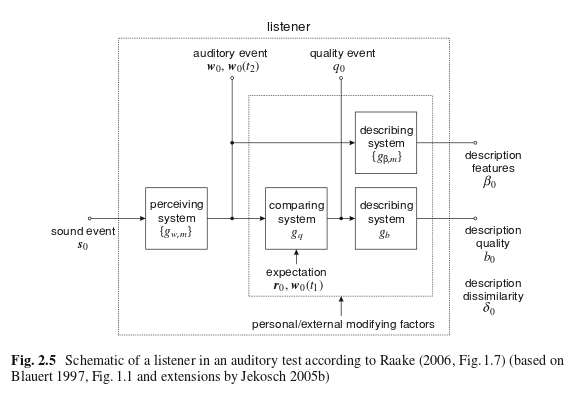
\includegraphics[width=1\textwidth]{figure/quality-event}
%	\caption{Quality formation and description process as extension to the perceptual event taken from \cite{waltermann_dimension-based_2013} after \cite{raake_short-_2006}.}
%	\label{img:chap02:quality-event} %Waeltermann, 2013
%\end{figure}

It is assumed that a perceptual event is evaluated by the \emph{comparing system} within an observer with regard to the \emph{quality features} of this event~\citet[\cf p. 17]{jekosch_voice_2005}.\footnote{\citet{jekosch_voice_2005} uses the term \emph{entity} with regard to the quality formation process.
As entity does not convey a temporal component, the term \emph{event} is in this work used instead following the notion of \citet{blauert_spatial_1996}.}

\begin{definition}[Quality Feature]
``A quality feature is a recognized and designated characteristic of an entity that is relevant to the entity's quality.''~\citep[][p. 17]{jekosch_voice_2005}
\end{definition}

It is assumed that the evaluation of the difference between the \emph{perceived quality features} and the \emph{desired quality features} result in the experienced quality~\citet[p. 23]{moller_quality_2014}.
With regard to telecommunication services and multimedia systems the term \emph{perceived quality} has been extended to \acf{QoE}.
In \ac{QoE} an observer is not regarded as a measurement instrument, but as an actor striving for a \emph{satisfying} perceived quality with regard to his expectations, requirements and needs.
In difference to an observer, who only describes an event, an actor that can react and also proactive make decisions.

\begin{definition}[\acf{QoE}]
``is the degree of delight or annoyance of a person whose experiencing involves an application, service, or system.
It results from the person’s evaluation of the fulfillment of his or her expectations and needs with respect to the utility and / or enjoyment in the light of the person’s context, personality and current state.''~\citep[][p. 19]{raake_quality_2014}.
\end{definition}

\citet{raake_speech_2006} and \citet{raake_quality_2014} extended the \emph{quality formation process} of \citet{jekosch_voice_2005}.
Here an anticipation and update process is added, which incorporates current experiences into the desired features affecting following experiences.
In addition, the concept of \emph{assumed quality} is derived.
\begin{definition}[Assumed Quality]\label{def:assumedquality}
``corresponds to the quality and quality features that users, developers, manufacturers or service providers assume regarding a system, service or product that they intend to be using, or will be producing, without however grounding these assumptions on an explicit assessment of \textit{quality based on experiencing}.''~\citep[][p. 17]{raake_quality_2014}.
\end{definition}
Here the experience has not taken place, but the quality formation process is based on expectations and prior knowledge.
Based upon \emph{assumed quality} a user might decide to initiate an interaction or rather avoid it.

The actual experience and resulting perceived quality is affected by influence factors.
\begin{definition}[Influence Factor]
Any characteristic of a user, system, service, application, or context whose actual state or setting may have influence on the \ac{QoE} for the user.~\citep[][p. 56]{reiter_quality_2014}
\end{definition}
Especially contextual factors, which include task, user behavior, and usage situation including location ~\citep[\cf,][p. 56]{reiter_quality_2014}, are important as those are often not invariant and affect the quality formation process.
For example high delay might not be noticed in a two-party telephone conversation, if only one speaker is talking.

\subsection{Assessment Methods}
For the assessment of \ac{QoE} experiments are conducted that are similar to psychophysical experiments allowing an actor to experience a system/service.
Information about the quality of the experience can be derived by monitoring the actor, observing his behavior, or requesting to describe his experience.

For a quantitative description often \ac{ACR} or \ac{CCR} scales are used allowing an actor to describe his experience (or parts of it) on a labeled scale.
Most prominent is the 5-point \ac{ACR}\footnote{This scale is often denoted as \ac{MOS} scale. This however is not correct as the \ac{MOS} is rather the combination of multiple judgments by one or more actors into one score by calculating the arithmetic mean.} ranging from \emph{Bad (1)} to \emph{Excellent (5)}.
The labels act as anchors, so multiple judgments of the same or different stimuli can be related with each other.
%Note that the term stimulus is misleading as it suggests an observer rather than an actor, which in some cases might be correct but not in general.

Based upon the judgments a \ac{MOS} can be derived that is assumed to describe the judgment of an \emph{average actor}.
Judgments can either be taken during the experience, which is denoted as \emph{momentary judgment}, or after an experience denoted as \emph{retrospective judgment}~\citep[\cf,][]{weiss_temporal_2014}.
Momentary judgments might affect the perception and quality formation process, but allows to investigate the impact of varying performance especially with regard to noticeability.
A retrospective judgment requires, however, that characteristics about the experience can be memorized while experiencing and later recalled for the judgment.
However, it has been observed that not all parts of an experience affect a retrospective judgment in a similar manner (\cf, \autoref{chap:04}).
%For the investigation of the impact of small differences between stimuli often paired comparison methodologies are applied, which present multiple stimuli and request to judge them with regard to each other or select the \emph{better} one.

It must be noted that a judgment cannot be considered as \emph{absolute} in terms of universal, because it is the result of the quality formation process and decription process.
These processes are affected by differences in the so-called internal reference, which might lead to biases \citep[\cf,][]{zielinski_biases_2008, pitrey_aligning_2011}.
For example the presentation of narrowband speech stimuli are judged better on the same scales, if no wideband stimuli are presented \citep[\cf,][]{koster_comparison_2015}.

\subsection{Prediction}
One major goal of research on \ac{QoE}, beyond understanding the underlying processes in detail, is the algorithmic prediction of judgments.
This is especially important as the evaluation by human actors is a rather expensive procedure limiting the number of evaluations.
Such a model can be applied for automatic evaluation, which is for example is useful for  development of new lossy coding algorithms.

A model receives maps the input, often a stimulus or an abstract reduced presentation of a stimulus, to an expected judgment.
%A model is in general created based upon judgments of human actors, often in terms of \ac{MOS}.
For speech transmission \ac{POLQA} \citep{itu-t_p.863:_2014} and \emph{E-Model} \citep{itu-t_g.107:_2014} are widely used examples.
Where as the former predicts perceived quality based upon the difference between input signal and output signal, the latter uses only a parametric, reduced representation.
Depending on the purpose of a model, different input and outputs are desired.
Input might also include beside technical performance-related characteristics, information about the influence factors.

However, a model is limited to the underlying data that lead to the selection of the model parts and parameters.
As those judgments were taken from a limited number of human actors in a specific situation for a \emph{limited} set of stimuli, a model must be carefully applied to the implied restrictions.
Using it outside its designed scope, might result in invalid predictions.